\begin{sidewaysfigure}[htbp]
\centering 
  \subfloat[Low friction, average velocity.]
  {
	  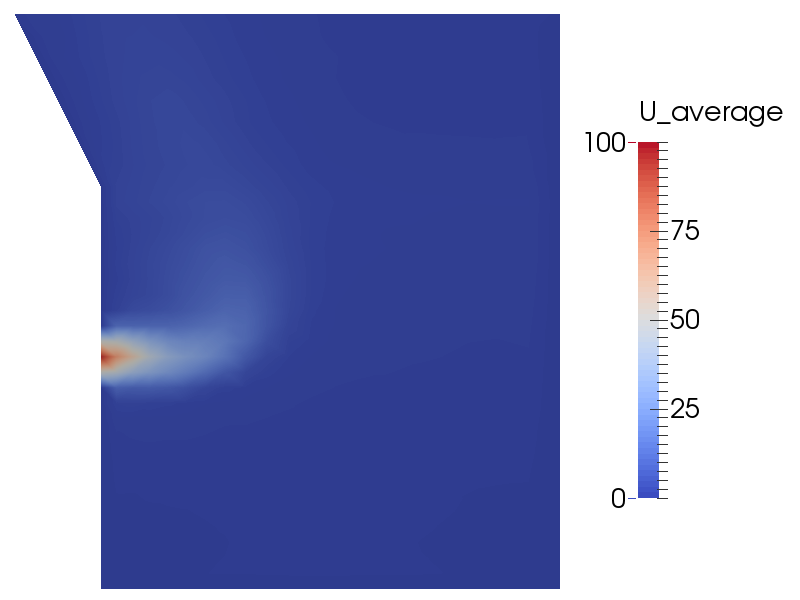
\includegraphics[width=.32\columnwidth]{images/227u_average_lf}
	  \label{fig:227u_average_lf}
  }
  \quad
    \subfloat[High friction, average velocity.]
    {
	  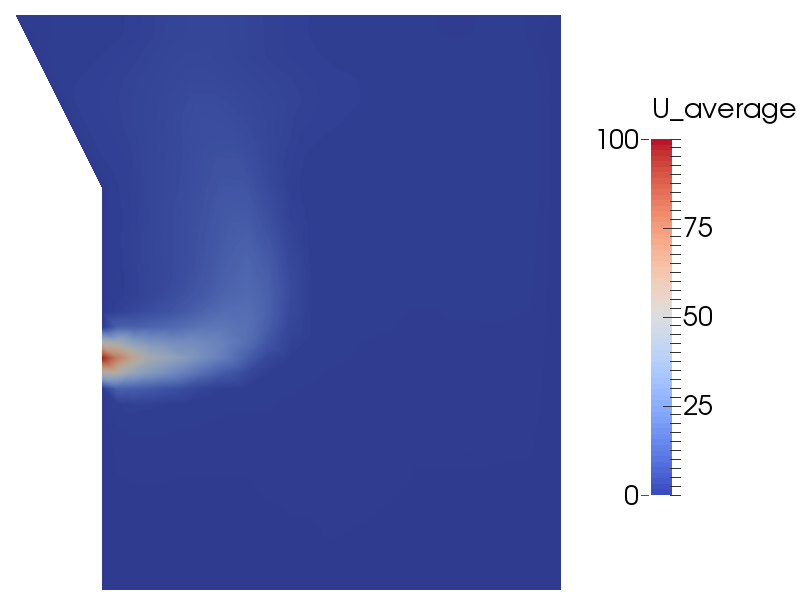
\includegraphics[width=.32\columnwidth]{images/226u_average_hf}
	  \label{fig:226u_average_hf}
  }
  \quad
    \subfloat[High friction, average velocity.]
    {
	  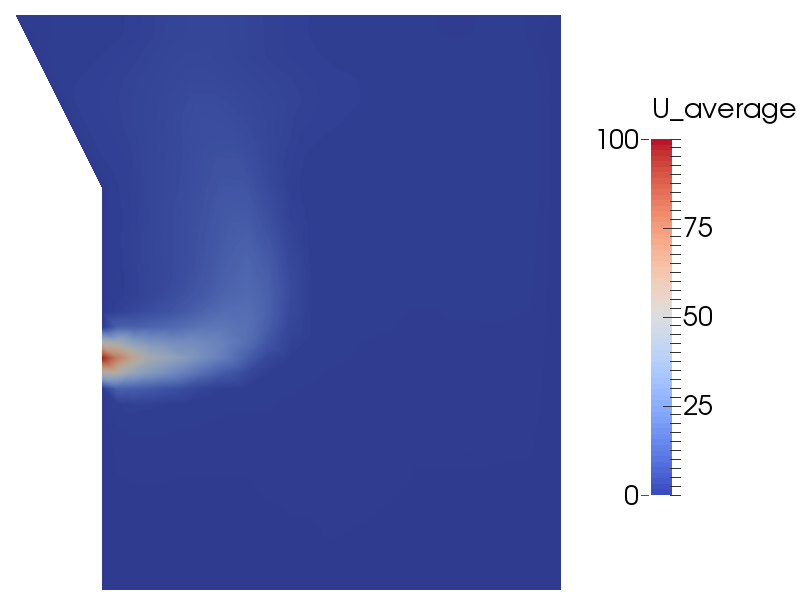
\includegraphics[width=.32\columnwidth]{images/226u_average_hf}
	  \label{fig:226u_average_hf}
  }
  \\
  \subfloat[Low friction, standard deviation velocity.]
  {
	  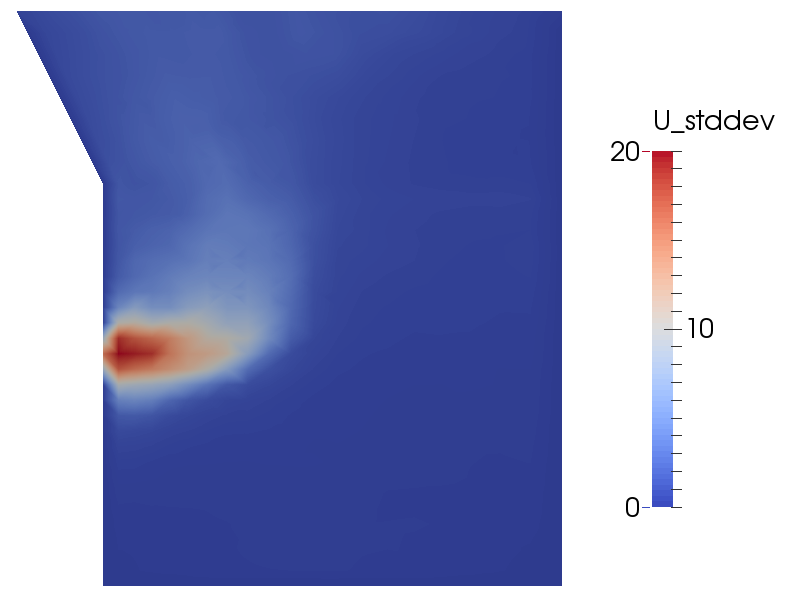
\includegraphics[width=.32\columnwidth]{images/229u_std_lf}
	  \label{fig:229u_std_lf}
  }
  \quad
    \subfloat[High friction, standard deviation velocity.]
    {
	  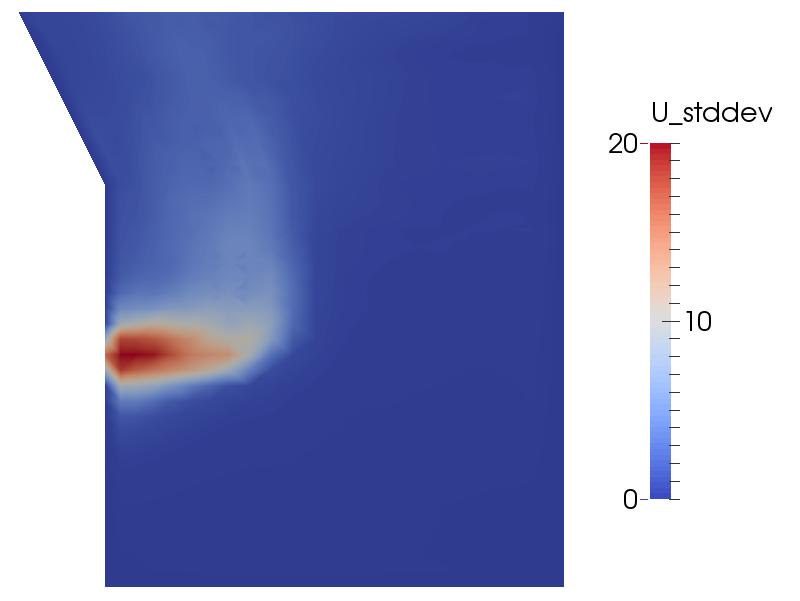
\includegraphics[width=.32\columnwidth]{images/228u_std_hf}
	  \label{fig:228u_std_hf}  }
  \\
  \caption{Fluid velocity with different sliding friction coefficient.}
  \label{fig:225racewayu}
\end{sidewaysfigure}